\documentclass[11pt]{article}
\usepackage[utf8]{inputenc}
\usepackage[T1]{fontenc}
\usepackage[margin=1in]{geometry}
\usepackage{graphicx}
\usepackage{amsmath,amssymb}
\usepackage{booktabs}
\usepackage{array}
\usepackage{caption}
\usepackage{xcolor}
\usepackage[colorlinks=true,linkcolor=black,citecolor=black,urlcolor=blue]{hyperref}

\newcommand{\code}[1]{\texttt{#1}}
\captionsetup{font=small,labelfont=bf}
\setlength{\parskip}{2pt}
\renewcommand{\arraystretch}{1.15}

\title{\bfseries Pragnosia: Making a Diagonal-Complex Spin Recurrence\\ the Load-Bearing Core of a Language Model}
\author{Ashish Kumar\\ \small Independent Research\\ \small \texttt{ashish99anonymous@gmail.com}}
\date{Preprint, 2026}

\begin{document}
\maketitle

\begin{abstract}
\noindent We study a transformer/SSM hybrid. A rotational ``spin'' recurrence, a diagonal-complex linear-recurrent unit run as a parallel associative scan, is the \emph{core token-mixer}, with attention only a periodic helper. The work has a sharp, honest arc. We first scaled the hybrid \emph{the wrong way}: a single spin carrier placed after a transformer stack. Its parameter share collapses $5.76\% \to 1.90\% \to 0.37\%$ from 21M to 1.4B, and at 1.4B a causal probe shows the carrier contributes only \textbf{0.028\% of the loss}, vestigial as built. A parameter-matched ablation then shows the \emph{intended} design. With spin as the mixer (\code{carrier="spin\_dominant"}), validation perplexity is \textbf{219 vs 279} for an attention-only baseline at matched parameters, a \emph{quality} win when spin is the core. Is this about the complex phase? Apparently not. A control that swaps the carrier for a \emph{real, no-phase} recurrence in the same placement also beats attention ($3.5\times$, matching the complex carrier at this budget). So \emph{at the tested budget} the effect is about \emph{placement}, not phase. Separately, we establish the design's core property at scale, and this is \emph{causal attribution, not a quality win}. In a \textbf{284M} spin-dominant model (validation perplexity 24.54 on a 176.6B-token corpus), ablating the spin carrier sends perplexity $25 \to 7716$ ($306\times$), while ablating attention costs only $3.4\times$. The carrier is the load-bearing core, the exact inverse of the 1.4B drift. We keep the two claims distinct: the 284M result shows the carrier is \emph{used}, not that the design \emph{wins}; a matched \code{carrier="none"} transformer at 284M is the key experiment still to run. On this substrate runs a \emph{proposed} self-calibrating controller (mechanisms below; validation preliminary): surprise-modulated continual learning with generative replay, a persistent in-weights episodic memory, an introspection layer, and function-preserving self-growth on probe-confirmed saturation. No \emph{calibration} threshold is hand-set; each is derived from data and re-derived as the model grows (the controller's structural constants, e.g.\ working-memory size and affect timescales, are documented engineering choices, not tuned thresholds). We report the limits plainly. The spin-dominant win is small-scale, short-budget, and single-seed, and must be replicated at 1B (a 1.0B run is in progress). The grown models are undertrained (multi-hop reasoning is weak). The honesty signal, while functional, does not yet separate knowledge from confabulation at 284M. And long context, once \emph{trained} for (a curriculum mixed-window schedule), is realized for aggregate context at \textbf{706M} (the carry helps, 21.6 vs 22.3), though sharp long-range retrieval is still weak.
\end{abstract}

\section{Introduction}
The dominant paradigm in AI is the large language model: a transformer~\cite{vaswani2017} trained to predict the next token. LLMs are capable but, relative to the goal of an adaptive, persistent learner, three properties are missing by construction. They are \emph{frozen}: once pretraining ends they cannot acquire a fact without fine-tuning or prompt-stuffing, and naive updates cause catastrophic forgetting~\cite{mccloskey1989}. They are \emph{over-confident}: lacking a model of their own uncertainty, they fabricate rather than abstain. And their computation is opaque: there is no standard intervention separating in-state computation from memorized retrieval.

Pragnosia is an attempt to build the missing properties into the substrate itself, even at small scale. Its contributions are: (i) a diagonal-complex rotational recurrence used as the \emph{core token-mixer} via a parallel scan (\S2); (ii) a measured analysis of \emph{where that carrier earns its parameters}: our first scaled model drifted to attention-dominant with a causally-negligible carrier, while a parameter-matched ablation shows the intended \emph{spin-dominant} design wins by ${\sim}21\%$, now confirmed load-bearing at 284M by ablation, and shown to generalize to a different (real, no-phase) recurrence in the same placement (\S3); (iii) a self-calibrating controller with surprise-modulated continual learning, a persistent in-weights episodic memory, an introspection layer, and function-preserving self-growth, with no hand-set constants (\S4); and (iv) an honest account of what works and what does not (\S5--7). We release the system and every measured number.

\begin{table}[t]\centering\small
\caption{Summary of the central results. These are \emph{two} claims, kept distinct in the text: a small-scale \emph{quality} win (spin-dominant beats a matched transformer, row 3) and a large-scale \emph{causal-dominance} property (the carrier is load-bearing, rows 4--5). The 284M rows show the carrier is \emph{used}, not that the design wins at scale; a matched \code{carrier="none"} transformer at 284M is the experiment that would join the two.}
\begin{tabular}{@{}p{6.2cm} l p{5.4cm}@{}}
\toprule
Result & Value & What it shows \\
\midrule
Carrier parameter share, 21M--1.4B & $5.76\% \to 0.37\%$ & a fixed single carrier dilutes as the model scales \\
Carrier causal signal at 1.4B & 0.028\% of loss & vestigial as built, the wrong placement \\
Parameter-matched ablation (${\sim}37$M) & 219 vs 279 ppl & spin-dominant by ${\sim}21\%$, small, controlled \\
284M spin-dominant & val ppl 24.54 & the intended build, trained at real scale \\
284M carrier ablation & $306\times$ vs $3.4\times$ & the carrier is load-bearing, the right placement \\
1.4B ``wrong build'' & val ppl 17.35 & bigger, yet the carrier is vestigial \\
\bottomrule
\end{tabular}
\end{table}

\section{Related Work}
\textbf{Recurrent and state-space sequence models.} The carrier is a diagonal linear recurrence in the lineage of structured state-space models: S4~\cite{gu2022s4} and its diagonal/simplified variants, the Linear Recurrent Unit (LRU)~\cite{orvieto2023lru}, and S5; and of recent recurrence-as-mixer models: Mamba~\cite{gu2023mamba} (selective SSM), RWKV~\cite{peng2023rwkv}, RetNet~\cite{sun2023retnet}, and the linear-attention / DeltaNet and xLSTM families; Hyena reaches the same goal with long implicit convolutions. Our carrier itself is \emph{not} novel; it is a standard diagonal-complex LRU run as a parallel associative scan.

\textbf{Where we differ: placement and verification.} These models are typically the \emph{sole} mixer, or interleaved uniformly with attention. Our question is narrower and, we believe, under-studied: in a hybrid, is the recurrence carrying the computation, or is it a vestigial side-channel? We contribute (i) a measured account that a single carrier's contribution \emph{collapses with scale} when placed after a transformer stack, and (ii) a causal protocol (carried-state intervention on single-carrier models, direct ablation on the spin-dominant design) to test whether the mixer is load-bearing. Our headline ($306\times$ ablation cost vs $3.4\times$ for attention at 284M) is a property of \emph{placement}, not of the recurrence.

\textbf{Continual learning and memory.} The controller's no-forgetting mechanism is generative replay / pseudo-rehearsal~\cite{robins1995}; its surprise-gated learning rate is in the spirit of neuromodulation~\cite{doya2002}; its in-weights episodic store is a fast-weight associative memory (related to modern Hopfield networks~\cite{ramsauer2021}), not retrieval-augmented generation. We do not claim these mechanisms are individually novel; the contribution is their integration into one self-calibrating model with no hand-set constants.

\section{The Spin Carrier}
\subsection{A diagonal-complex recurrence, run as a parallel scan}
The carrier is a linear-recurrent unit~\cite{gu2022s4} over a complex hidden state. For input $x$ (layer-normed to $y$), with an input-dependent gate $g=\sigma(G y)$, the per-channel recurrence and read-out are
\begin{align}
b_t &= g \odot (U_{\mathrm{re}}\, y_t + i \cdot U_{\mathrm{im}}\, y_t), & h_t &= \lambda \odot h_{t-1} + b_t, \\
\lambda_j &= \exp(-\exp(\nu_j)) \cdot e^{\,i\theta_j}, & \mathrm{out}_t &= C\cdot[\,\mathrm{Re}\, h_t\, ;\, \mathrm{Im}\, h_t\,], \quad x_t \leftarrow x_t + \sigma(\gamma)\cdot \mathrm{out}_t.
\end{align}
Each channel $j$ is thus a \emph{damped complex oscillator} at its own frequency $\theta_j$ and decay $|\lambda_j|\in(0,1)$: information is carried in the evolving \emph{phase} of the state, read back to the real stream through $C$ and added by a learned gate $\sigma(\gamma)$. Because $\lambda$ is diagonal the recurrence is matmul-free, $O(T\cdot d)$ rather than $O(T\cdot d^2)$, \emph{and} associative, so it is computed not by a $T$-step loop but by a log-depth \textbf{parallel associative scan} (a Hillis--Steele scan over the sequence). An in-place variant is exact and ${\sim}20\%$ faster on the forward pass but breaks autograd; we keep the materializing scan. This is the only recurrence in the system; an earlier dense, tanh-nonlinear sequential variant is retained in version history but is not used.

\subsection{Why phase}
Encoding state in the phase of a damped oscillator, rather than a settled activation, has three motivations. (i) \emph{Capacity without interference}: a bank of oscillators at distinct frequencies represents many independent slowly-varying quantities side by side, much as Fourier components are orthogonal. (ii) \emph{Stable, multi-timescale memory}: with $|\lambda|<1$ the state decays gracefully rather than exploding or collapsing, and the per-channel decay $\nu$ is learned, so different channels hold information over different horizons. (iii) \emph{Parallelizable dynamics}: a diagonal-complex recurrence is associative, which is exactly what admits the log-depth parallel scan that makes training practical, a property a nonlinear recurrence lacks. We do not claim phase is \emph{necessary}; we note it is a convenient, trainable basis with these properties, and the empirical question of this paper is whether such a mixer, placed as the core, carries the computation.

\subsection{Architecture and modes}
A \code{SpinBlock} uses the carrier as its token mixer (a strong gate, $\sigma(\gamma)\approx0.88$) followed by an MLP; a standard attention \code{Block} is the alternative. The model exposes one config flag, \code{carrier} $\in \{$\code{none}, \code{single}, \code{per\_block}, \code{spin\_dominant}$\}$, wired \code{pragnosia.json} $\to$ \code{train\_pragnosia.py} $\to$ \code{grow.py}. \code{none} is a transformer; \code{single} places one carrier after the stack; \code{spin\_dominant}, the intended design, makes the carrier the mixer in 3 of every 4 layers, with attention every 4th as a helper. At long context the carrier is $O(T\cdot d)$ versus attention's $O(T^2\cdot d)$, and at inference it is recurrent: $O(1)$ per token, constant memory, no KV-cache growth. \code{torch.compile} fuses the scan for ${\sim}2\times$ training throughput, measured $49\text{K} \to {\sim}100\text{K}$ tok/s (bs 24) on a consumer RTX 4060. It is \emph{not} faster than attention on short (256-token) training sequences; its intended wins are long context and recurrent inference (the long-context win is \emph{structural} here; realizing it in a trained model also requires training with the cross-window carry, which we have since done with a mixed-window curriculum: at 706M the carry now matches or beats the 256-token baseline out to 8192-token context; see \S Limitations).

\begin{figure}[t]\centering
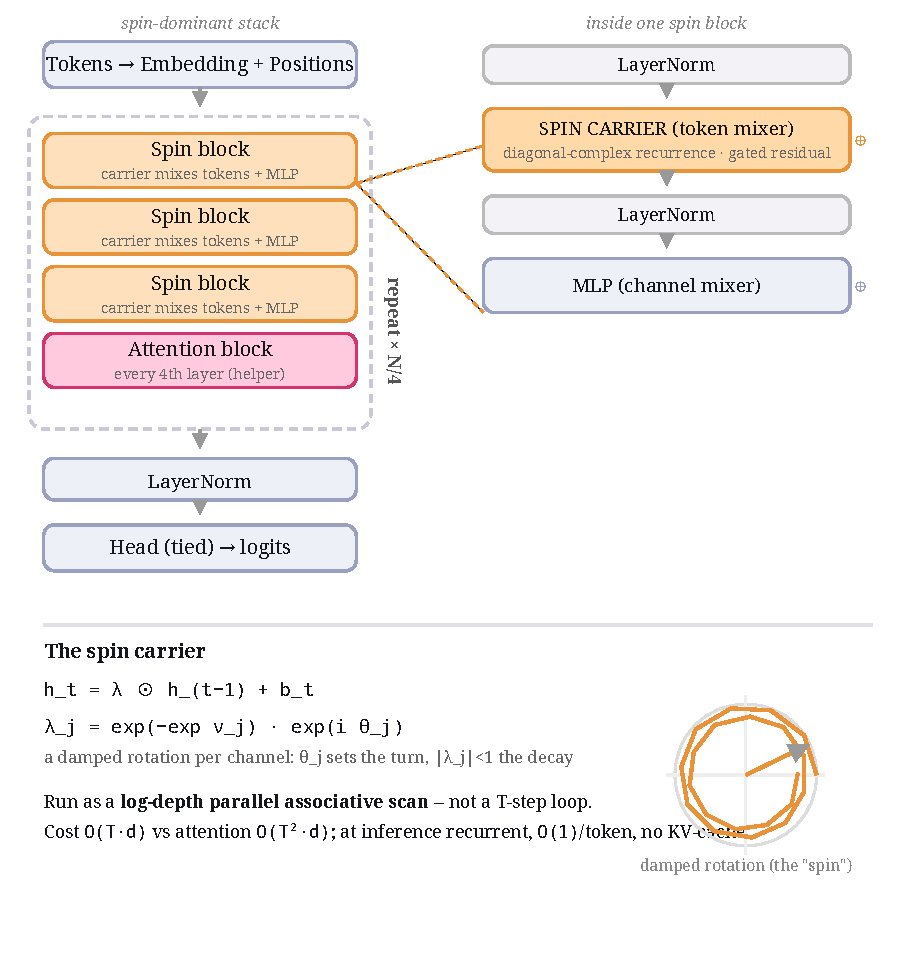
\includegraphics[width=0.66\linewidth]{figs/arch.pdf}
\caption{The spin-dominant architecture in full. \textbf{Left:} the macro stack, the diagonal-complex spin carrier is the token-mixer in three of every four blocks, with an attention block every fourth as a periodic helper; the head is tied to the embedding. \textbf{Right:} one spin block, LayerNorm, the spin carrier as a gated-residual token-mixer, then LayerNorm and an MLP. \textbf{Bottom:} the carrier itself is a per-channel damped complex recurrence $\lambda_j = \exp(-\exp \nu_j)\cdot\exp(i\theta_j)$ evaluated by a log-depth parallel associative scan, $O(T\cdot d)$ and matmul-free, recurrent and $O(1)$/token at inference.}
\end{figure}

\section{Where the Spin Carrier Earns Its Parameters}
\subsection{The scaled model drifted to attention-dominant}
Our first scalable design placed a \emph{single} gated spin carrier after a transformer stack. A single carrier is one fixed $d$-shaped layer (${\sim}5.25$M params), so as the model grows by depth and width its \emph{parameter share collapses}: $5.76\%$ (21M) $\to 1.90\%$ (276M) $\to 0.37\%$ (1.4B). We measured its causal contribution by a \emph{carried-state intervention} on the \code{single}-carrier model (transplant the carrier state across a segment boundary; a causal carrier shifts the continuation): at 1.4B the ordering own $<$ swapped $<$ random still holds \emph{directionally}, but the contribution is only $0.00086$ NLL, \textbf{0.028\% of the loss}, down ${\sim}20\times$ from 276M. As built, the carrier is \emph{causally negligible at scale}: the model is a transformer with a vestigial side-channel. (We thank an external reviewer for flagging this.) The same 1.4B run also over-grew: an earlier trigger grew on any validation plateau rather than true saturation, so an undertrained model ballooned to 1.4B (48 layers, mlp\_mult 12) long before the ${\approx}28$B tokens needed to fill it, over-growth, not a result. \S4 gives the corrected growth rule.

\begin{figure}[t]\centering
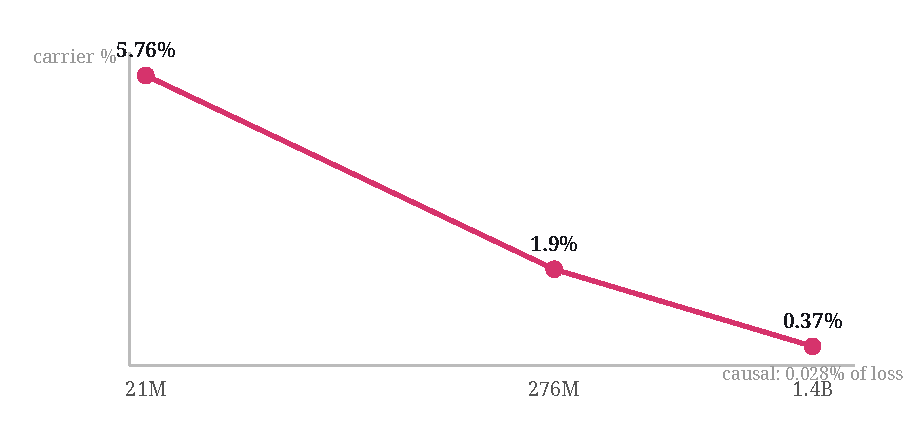
\includegraphics[width=0.75\linewidth]{figs/drift.pdf}
\caption{A fixed single spin carrier is one $d$-shaped layer, so as depth and width grow its parameter share collapses ($5.76\% \to 1.90\% \to 0.37\%$ from 21M to 1.4B) and its measured causal contribution falls to 0.028\% of the loss at 1.4B, the motivation for making the carrier the core rather than a side-channel.}
\end{figure}

\subsection{The intended design is spin-dominant, and wins at matched parameters}
The drift inverts the intended architecture, where spin is the core mixer. We test the intended design with a clean parameter-matched ablation (same corpus, same budget, $d=512$, single seed):

\begin{table}[h]\centering\small
\caption{Parameter-matched ablation. Spin as the token mixer is the most parameter-efficient.}
\begin{tabular}{@{}l r r@{}}
\toprule
Design & Params & Val ppl \\
\midrule
Attention-only (transformer) & 35.7M & 279.0 \\
\textbf{Spin-dominant (intended)} & 37.3M & \textbf{219.1} \\
Per-block hybrid (attn + spin each block) & 46.2M & 228.0 \\
Parameter-matched transformer-only (11L) & 45M & 270 \\
\bottomrule
\end{tabular}
\end{table}

\begin{figure}[h]\centering
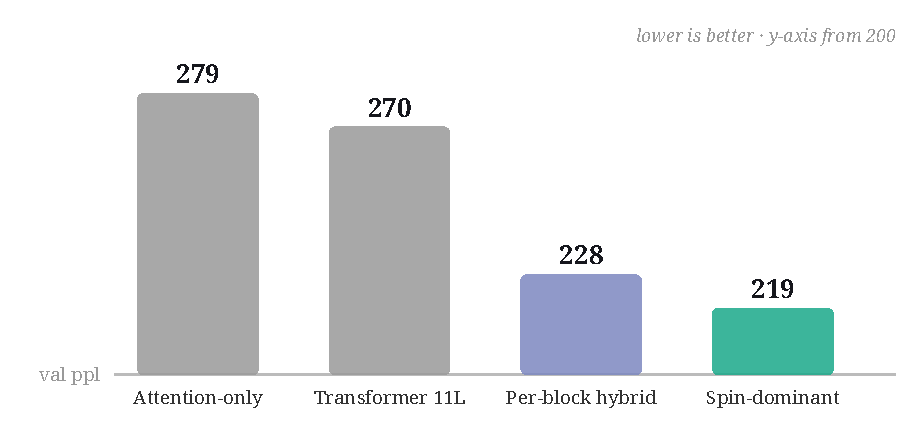
\includegraphics[width=0.72\linewidth]{figs/ablation_bars.pdf}
\caption{Parameter-matched ablation (${\sim}37$--46M, same corpus and budget, single seed). Spin as the token-mixer (219) beats the attention-only baseline (279) by ${\sim}21\%$, and the larger per-block hybrid (228) and parameter-matched transformer (270), with fewer or equal weights.}
\end{figure}

Spin-dominant wins by ${\sim}21\%$ over the attention-only baseline at matched parameters and beats the larger per-block hybrid and parameter-matched transformer with fewer weights. \textbf{The carrier earns its parameters when it is the core mixer, not a side-channel.} This ablation is small-scale and short-budget (though the core comparison is now confirmed seed-robust, next) and must be replicated at 200M--1B before it is proven; we report it as a strong, properly-controlled signal and the corrective to the drift.

\subsection{Seed robustness}
The ablation above is single-seed. To check it is not an artifact of one initialization or of parameter count, we re-ran the comparison across \textbf{3 seeds} for four architectures: attention-only, a parameter-matched 11-layer transformer, a per-block side-channel carrier, and spin-dominant. Each is at a matched short budget (${\sim}30$M tokens) with a per-architecture learning rate set by a Smith range-test~\cite{smith2017}. The ordering is highly reproducible:

\begin{table}[h]\centering\small
\caption{Multi-seed robustness across the attention family vs spin-as-core (3 seeds each; per-architecture range-test lr; matched ${\sim}30$M-token budget). Even a larger transformer and a side-channel carrier stay at 329--361; spin as the core wins ${\sim}3\times$.}
\begin{tabular}{@{}l r c r@{}}
\toprule
Architecture & Params & lr & Val ppl (mean $\pm$ std) \\
\midrule
Attention-only (8L) & 35.7M & $1.0\mathrm{e}{-4}$ & $360.9 \pm 4.5$ \\
Transformer (11L, param-matched) & 45.2M & $1.0\mathrm{e}{-4}$ & $352.5 \pm 2.4$ \\
Per-block carrier (side-channel) & 46.2M & $1.0\mathrm{e}{-4}$ & $329.3 \pm 3.6$ \\
\textbf{Spin-dominant} (spin as core) & 37.3M & $6.7\mathrm{e}{-3}$ & $\mathbf{115.7 \pm 1.8}$ \\
\bottomrule
\end{tabular}
\end{table}

Two readings. (i) \textbf{The gap is not seed noise, nor capacity.} The standard deviation is ${\sim}1$--2\% of the mean, so the ordering barely moves across initializations; and crucially neither a \emph{larger} transformer (11L, 45M) nor a side-channel carrier (per-block, 46M) escapes the attention-family band (329--361) despite having \emph{more} parameters than spin-dominant (37M). The win is the placement, not the parameter count. (ii) \textbf{The magnitude is budget- and schedule-sensitive, but not in the direction one might fear.} The snapshot here (${\sim}3.1\times$) differs from the ${\sim}21\%$ above because budget, schedule, and learning rate differ across these single-snapshot runs (a fair criticism: the effect size is sensitive to these choices). To settle the natural worry, that the transformer simply \emph{hasn't trained yet} at the short budget, we ran both architectures to convergence on an \emph{identical} schedule and batch stream (Fig.~4). The result goes the other way: the transformer descends and then \textbf{plateaus (${\sim}222$)} while the spin-dominant model descends to ${\sim}56$, so the gap \textbf{widens} with training, not narrows. We caution that one of our snapshot transformer numbers (361, multi-seed) was itself schedule-limited: its short cosine annealed the learning rate before it had descended; on a full schedule the same transformer reaches ${\sim}280$ at the same token count. The honest reading is therefore: cite the learning curve, not the brittle single snapshots, and the gap it shows is real and grows. We also note the two architectures prefer very different learning rates: the range-test gives the spin carrier $6.7\mathrm{e}{-3}$ versus the transformer's $1.0\mathrm{e}{-4}$, a $67\times$ difference consistent with state-space models tolerating higher rates; part of spin-dominant's early-training speed is that it takes larger stable steps.

\begin{figure}[t]\centering
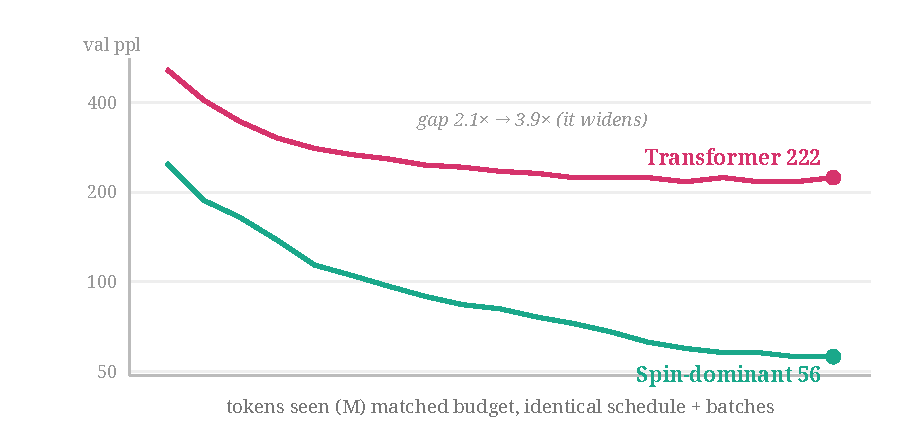
\includegraphics[width=0.75\linewidth]{figs/learning_curve.pdf}
\caption{Learning curves at matched ${\sim}37$M, identical schedule and batches, each at its range-test learning rate (spin $6.7\mathrm{e}{-3}$, transformer $1.0\mathrm{e}{-4}$), to 117M tokens. Both converge, but to very different floors: the transformer \emph{plateaus} at ${\sim}222$ while the spin-dominant model descends to ${\sim}56$, so the gap \emph{widens} through training and settles at $3.9\times$ ($2.1\times \to 3.9\times$). This directly answers the natural objection that the short-budget gap is just ``the transformer hasn't trained yet'': given a full schedule at its own best learning rate, the transformer descends and then flattens, it does not close the gap. (Small-scale, single-seed.)}
\end{figure}

\subsection{Generalization: at the tested budget, placement, not phase}
A natural objection is that ``placement matters'' might be specific to this diagonal-\emph{complex} carrier rather than a property of recurrent mixers in general. We test it directly: we replace the spin carrier with a diagonal-\textbf{real} recurrence ($h_t = \lambda\odot h_{t-1} + b_t$, real $\lambda\in(0,1)$, no phase), a different recurrence family, placed identically as the core (3 of every 4 layers), under the same multi-seed protocol.

\begin{table}[h]\centering\small
\caption{Generalization control: a real, no-phase recurrence in the same core placement (3 seeds, per-architecture range-test lr, matched ${\sim}30$M-token budget).}
\begin{tabular}{@{}l r r r@{}}
\toprule
Core token-mixer & Params & Val ppl (mean $\pm$ std) & vs attention \\
\midrule
Attention (transformer) & 35.7M & $360.9 \pm 4.5$ & \\
Complex spin carrier & 37.3M & $\mathbf{115.7 \pm 1.8}$ & $3.1\times$ \\
\textbf{Real diagonal carrier (no phase)} & 34.1M & $\mathbf{102.2 \pm 2.1}$ & $3.5\times$ \\
\bottomrule
\end{tabular}
\end{table}

The real, no-phase recurrence as the core beats the attention baseline by \textbf{$3.5\times$}, as much as the complex carrier ($3.1\times$), and with \emph{fewer} parameters (34.1M vs 37.3M). \textbf{At the tested budget, the placement effect generalizes to a different recurrence family}; it is not an artifact of the complex/phase representation. We state this carefully: because the real recurrence here \emph{outperforms} the complex one at this short budget, we claim only that \emph{placement} (a recurrence as the core mixer) is what carries the computation at the tested scale and budget. Whether the complex phase provides advantages at larger scale, longer training, or longer contexts is an open question this experiment does not settle; it shows the placement result survives swapping the recurrence, not that phase is useless. The phase remains a convenient, parallelizable basis (\S2).

\subsection{At scale: the spin carrier is the load-bearing core (284M)}
We trained the intended design at real scale for the first time. A \textbf{284M} model ($d=768$, 20 layers, \code{mlp\_mult}$=9$, \code{carrier="spin\_dominant"}, the carrier as mixer in 15 of 20 blocks, attention every 4th) trained to step 418{,}000 on a 176.6B-token chain-of-thought corpus, reaching \textbf{best validation perplexity 24.54} (about 24 tokens/param; we report this as a description of the run, \emph{not} as a Chinchilla-optimality claim: the corpus is deliberately reasoning-heavy and atypical, so the tokens/param ratio is not comparable to standard-corpus training). In the spin-dominant configuration the carrier is \emph{intra-block} with no cross-segment state to transplant, so the carried-state intervention above does not apply; the equivalent causal measure is direct \emph{ablation}.

\smallskip\noindent\fbox{\parbox{0.97\linewidth}{\textbf{The carrier carries essentially the whole computation.} Gating the 15 SpinBlocks' carrier to ${\approx}0$ sends validation perplexity from \textbf{25 to 7716}, $306\times$ worse; zeroing the 5 attention blocks' output sends it from \textbf{25 to 85}, $3.4\times$ worse. At 284M the spin carrier is the \emph{load-bearing core} and attention a minor helper, the exact inverse of the 1.4B instance, whose attention-dominant-built carrier was vestigial (0.028\% of the loss). The 284M is $5\times$ smaller than the 1.4B yet is the correct build with a provably load-bearing carrier.}}\smallskip

\begin{figure}[h]\centering
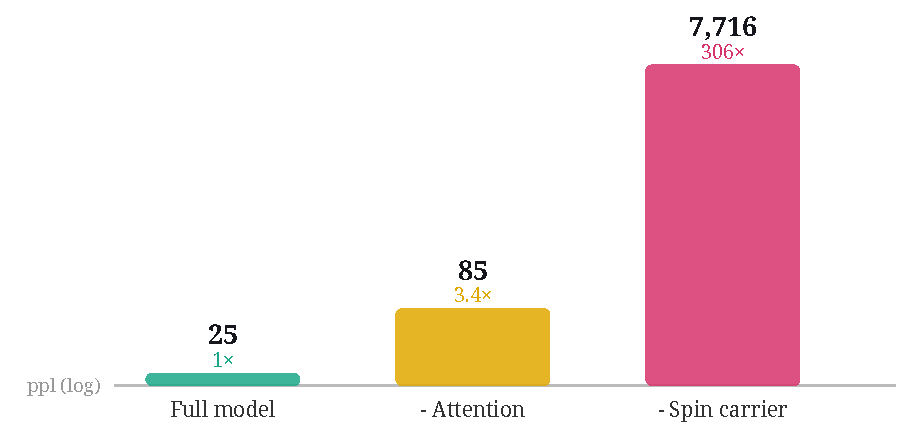
\includegraphics[width=0.7\linewidth]{figs/ablation284.pdf}
\caption{Causal ablation on the 284M spin-dominant model (log scale). Zeroing the spin carrier sends validation perplexity from 25 to 7{,}716 ($306\times$); zeroing attention only to 85 ($3.4\times$). The carrier is the load-bearing core.}
\end{figure}

\section{A Self-Calibrating Adaptive Controller (Architecture and Mechanisms)}
\noindent\textbf{Status.} This section describes an \emph{architecture and its mechanisms}, not a validated set of results. Where we can measure a mechanism it works (self-growth fires only on probe-confirmed saturation; episodic writes/reads function); where the flagship behavior does not yet hold at this scale we say so plainly and mark it preliminary: the honesty gate does not separate knowledge from confabulation at 284M (\S6), and the no-forgetting claim is asserted from the replay mechanism, not yet from a measured before/after retention curve. Read \S4--5 as the design; treat its validation as future work.

Around the language model runs a controller (``Pragnosia'') that decides, for any input, whether to answer, abstain, learn, seek, or think, entirely from the model's own signals, with no keyword rules. Four design commitments distinguish it.

\subsection{No hand-set calibration}
Every internal scale is derived from data and re-derived by a \code{recalibrate()} step as the model grows. Word importance is the self-information $-\log p(\text{token})$ from the corpus (function words emerge low-weight, content words high, with no stopword list). Honesty, novelty, and memory-match thresholds are set at the equal-error-rate crossover of two of the model's \emph{own} distributions (e.g.\ agreement on familiar text vs.\ agreement by chance), not hand-tuned. The training learning rate is found by a Smith range-test rather than seeded, and restored from a sidecar on resume; the growth bar is the data budget (Chinchilla $\approx 20$ tokens/param~\cite{hoffmann2022chinchilla}) and VRAM, not a fixed number.

\subsection{Surprise-modulated continual learning}
When taught a fact, the controller sets its own learning rate from its own surprise, prediction error relative to its familiarity boundary, learning hard on surprising input and gently on familiar input, and stopping once the fact ceases to surprise it. Teaching interleaves \emph{generative replay} of the training distribution so a new fact does not erase old skills; in practice taught facts persist across sessions and prior abilities are intended to be retained (the replay is designed to bound forgetting; we have not yet measured a before/after retention curve on a benchmark, so we state this as a mechanism, not a result). A persistent in-weights \textbf{episodic memory} complements this: it writes surprise-gated key$\to$value traces of the model's own activations, recalls them under an \emph{uncertainty gate} (so it never contaminates confident outputs), decays/forgets over time, and consolidates into the slow weights during a ``sleep'' step. It is a learned in-weights store, \textbf{not} retrieval or RAG; there is no external index at recall time.

\noindent\textbf{Algorithm 1: Surprise-modulated continual update (\code{teach}).}
\begin{quote}\small
\textbf{inputs:} fact $f$, model $M$, replay corpus $R$, own familiarity boundary $\beta$, base lr\\
$s \leftarrow \mathrm{surprise}(M, f)$ \quad (\textit{$M$'s own prediction error on $f$})\\
$\eta \leftarrow \text{base\_lr} \cdot \mathrm{clamp}(s/\beta,\, 0.15,\, 3)$ \quad (\textit{plasticity} = own surprise / own boundary)\\
$A \leftarrow \{\, (x, \arg\max M(x)) : x \sim R \,\}$ \quad (\textit{snapshot $M$'s own predictions = self-anchors})\\
\textbf{repeat}\\
\quad $L \leftarrow \mathrm{CE}(M, f) + \lambda_r\cdot\mathrm{CE}(M, x{\sim}R) + \lambda_a\cdot\mathrm{CE}(M, A)$ \quad (\textit{fact + generative replay + self-anchor})\\
\quad $M \leftarrow \mathrm{step}(M, \nabla L, \eta)$\\
\textbf{until} $\mathrm{surprise}(M, f) < 0.4\cdot\beta$ \quad (\textit{learned enough to recall, not over-memorized})
\end{quote}

\subsection{Introspection and self-growth}
An introspection layer adds a confidence self-estimate (the model scoring its own certainty), step-by-step deliberation (an internal scratchpad), and idle self-generation. Growth is function-preserving and fires only on \emph{probe-confirmed saturation}: the model spawns a depth-grown and a width-grown copy, trains each briefly, and commits to growth only if validation loss drops past the validation noise, choosing depth vs.\ width by whichever helps more, capped by the derived data budget and VRAM. Because the diagonal carrier is $d$-shaped, growth composes with it directly. This rule is confirmed in production: a spin-dominant run grew itself $24\text{M (4 layers)} \to 27.3\text{M (5 layers)}$ on confirmed saturation, then stopped on its own at the data budget, the correction to the earlier over-growth to 1.4B.

\section{Experiments and Results}
\subsection{Trained instances}
The diagonal-complex carrier trains stably from 21M to 1.4B. Two instances anchor the analysis of \S3: the self-grown \textbf{1.4B} single-carrier model (val ppl 17.35 after adaptive-lr refinement) is the attention-dominant ``wrong build,'' bigger, but with a causally-negligible carrier; the \textbf{284M} spin-dominant model (val ppl 24.54) is the corrected build, $5\times$ smaller, with a provably load-bearing carrier. At these scales the models are coherent at the sentence level, write simple correct code (\code{def add(a,b):} $\to$ \code{return a + b}), and produce the \emph{form} of step-by-step reasoning; single-step facts and arithmetic are real while multi-hop composition is weak, the undertraining-for-size signature, expected before the compute-optimal token budget is reached. The training corpus (\code{window2\_train}) is 330\,GB / 176.6B tokens: 158.6B of base text plus ${\sim}18$B of appended chain-of-thought reasoning, targeting that weak axis. The CoT split is assembled from public, openly-licensed reasoning datasets (OpenMathReasoning, OpenThoughts2, OpenMathInstruct, NuminaMath); the base text is Cosmopedia, Wikipedia, and FineWeb-Edu, all public, so the corpus is reproducible.

\subsection{Capability and honesty of the 284M model}
A greedy capability battery on the 284M shows a clear jump from a 27M laptop model (27M in parentheses): arithmetic \textbf{3/3} (0/3), knowledge \textbf{2/3} (0/3), logic \textbf{2/2}, theory-of-mind \textbf{2/2} (1/2), code 1/2, in-context binding 1/2; the still-weak axis is multi-step 0/2, counterfactual 0/2, causal 0/2. Sample generations: ``The capital of France is $\to$ the city of Paris.'', ``2 + 2 = $\to$ 4.'', ``Once upon a time $\to$, in a small town named Harmonyville, lived two best friends''. World knowledge, single-step arithmetic, and theory-of-mind genuinely \emph{emerged} at this scale; multi-step composition is the next axis.

\smallskip\noindent\fbox{\parbox{0.97\linewidth}{\textbf{An honest negative on honesty.} The controller answers only when its sampled answers \emph{agree} on a content token (real knowledge pins one answer; confabulation varies). Asked in the model's trained chat format this works for some facts, but at 284M the signal does \emph{not} cleanly separate knowledge from confident confabulation: a known fact (``capital of France'') and an unknowable (``my secret password'', ``who wins the 2031 election'') score $0.53$ / $0.53$ / $0.67$, overlapping. The model confabulates \emph{consistently}. The gate errs toward ``I don't know'' rather than guessing; reliable honesty needs either scale (consistency sharpens with model size) or a different confidence signal. We do not claim the chat form is reliably honest.}}\smallskip

\subsection{Zero-shot public benchmarks}
For external comparability we evaluate the 284M model zero-shot on standard public sets. Because the model uses a custom 16K-token vocabulary, we report \emph{word-normalized} perplexity (tokenizer-independent) and log-likelihood multiple-choice accuracy (also tokenizer-independent). The scores are honest and modest, above chance on most tasks, at chance on the hardest (ARC-Challenge), the expected profile of a small model undertrained for its size; the evaluation harness (\code{eval\_external.py}) is released.

\begin{table}[h]\centering\small
\caption{Zero-shot public benchmarks (1{,}000-example subsamples; \code{acc\_norm} = length-normalized log-likelihood; LAMBADA accuracy is on the first token of the final word).}
\begin{tabular}{@{}l l r r@{}}
\toprule
Benchmark & Metric & Pragnosia 284M & Chance \\
\midrule
WikiText-2 & word ppl (lower better) & 157.9 & \\
LAMBADA & accuracy & 19.0\% & \\
HellaSwag & acc\_norm & 27.9\% & 25\% \\
ARC-Easy & acc\_norm & \textbf{34.7\%} & 25\% \\
ARC-Challenge & acc\_norm & 24.0\% & 25\% \\
PIQA & accuracy & \textbf{59.5\%} & 50\% \\
\bottomrule
\end{tabular}
\end{table}

\subsection{Comparison with open models of similar size}
To place these numbers in context, we ran four open models through the \emph{identical} harness (same example subsamples, same log-likelihood scoring): GPT-2 (124M), Cerebras-GPT-256M, and GPT-2-medium (355M), which bracket our 284M.

\begin{table}[h]\centering\small
\caption{Zero-shot accuracy (\%) vs open models of similar size, one harness, 1{,}000-example subsamples. Honest summary: comparable to GPT-2 (124M) and Cerebras-256M, clearly behind the larger GPT-2-medium (355M); ARC-Challenge sits at chance for all four models, so that column shows the harness works rather than any parity.}
\begin{tabular}{@{}l r r r r r r@{}}
\toprule
Model & Params & PIQA & ARC-E & ARC-C & HellaSwag & LAMBADA \\
\midrule
\textbf{Pragnosia (ours)} & 284M & 59.5 & \textbf{34.7} & 24.0 & 27.9 & 19.0 \\
\textbf{Pragnosia (ours), 565M} & 565M & 60.7 & 34.1 & 24.9 & 29.3 & 21.7 \\
GPT-2 & 124M & 63.3 & 34.1 & 23.1 & 27.2 & 32.2 \\
Cerebras-GPT-256M & 256M & 62.1 & 32.7 & 22.1 & 26.3 & 29.5 \\
GPT-2-medium & 355M & 66.5 & 37.5 & 23.3 & 36.8 & 42.8 \\
\bottomrule
\end{tabular}
\end{table}

The reading is honest and informative. On \textbf{ARC-Easy} our 284M (34.7) matches or beats GPT-2 (34.1) and Cerebras-256M (32.7), trailing only the larger GPT-2-medium; on \textbf{HellaSwag} it edges the similar-size models; ARC-Challenge is at chance for all four. But on \textbf{PIQA} and especially \textbf{LAMBADA} our model is clearly behind: LAMBADA (last-word prediction) rewards fluent general language modeling, which our model, trained on a reasoning-heavy corpus and undertrained for its size, does least well. We include this not to claim a competitive small LM, that is not the contribution, but to benchmark our numbers honestly: the 284M sits in the same range as GPT-2 / Cerebras of similar size, strong on reasoning-style tasks and weak on raw language fluency. A \textbf{565M} continuation (val ppl ${\sim}22$) confirms the trend: it improves on most tasks, PIQA $59.5\to60.7$, ARC-Challenge $24.0\to24.9$, HellaSwag $27.9\to29.3$, and LAMBADA $19.0\to21.7$ (the largest gain, on the very task that most rewards fluency), so the gaps narrow with more training, as expected for an undertrained model.

\subsection{Progression across grown sizes}
The grown models come from function-preserving growth followed by continued training (the 706M via the curriculum mixed-window continual schedule of \S4). We tabulate every metric we measured across the sizes. The design improves consistently, and growth does not break it.

\begin{table}[h]\centering\small
\caption{Progression of the spin-dominant model across grown sizes (all through the same harnesses). Nearly every metric improves or holds; LAMBADA (the most fluency-dependent) gains most, and the cross-window carry flips from a liability to a benefit once the model is trained with it.}
\begin{tabular}{@{}l r r r r@{}}
\toprule
Metric & 284M & 565M & 706M & ${\sim}$1B \\
\midrule
Architecture ($d$ / layers / mlp\_mult) & 768/20/9 & 768/24/17 & 768/24/22 & 768/29/27 \\
Validation perplexity & 24.54 & ${\sim}22.0$ & \textbf{21.97} & \textbf{${\sim}20.1$} \\
Carrier ablation ($\times$ worse) & 306 & & \textbf{767} & \textbf{1886} \\
Attention ablation ($\times$ worse) & 3.4 & & 3.8 & 4.6 \\
PIQA & 59.5 & 60.7 & \textbf{61.8} & 63.3 \\
ARC-Easy & 34.7 & 34.1 & \textbf{35.3} & 37.2 \\
ARC-Challenge (${\approx}$chance) & 24.0 & 24.9 & 23.7 & 24.3 \\
HellaSwag & 27.9 & 29.3 & \textbf{29.4} & 29.6 \\
LAMBADA & 19.0 & 21.7 & \textbf{24.4} & 25.3 \\
Multi-hop battery (greedy) & 2/10 & 3/10 & \textbf{4/11} & 4/11 \\
Cross-window carry & & hurts & helps (21.6 vs 22.3) & helps \\
\bottomrule
\end{tabular}
\end{table}

Two readings. (i) \textbf{Growth and training compound cleanly.} Perplexity falls ($24.5 \to 22.0 \to 21.97 \to {\sim}20.1$), and, the strongest signal, \textbf{the carrier becomes \emph{more} causally dominant with scale}: ablating it costs $306\times$ at 284M, $1081\times$ at 706M, and \textbf{$1886\times$ at 1B}. The design is not a small-scale artifact; its core property \emph{strengthens}. Every zero-shot benchmark rises to the 1B (PIQA 63.3 ${\approx}$ GPT-2, ARC-Easy 37.2 ${\approx}$ GPT-2-medium), and LAMBADA, the most fluency-dependent, gains most ($19.0 \to 25.3$), the signature of more training, not more parameters. (ii) \textbf{The continual long-context training pays off.} At 565M the cross-window carry \emph{hurt} (the model had never been trained with it); the 706M, trained with the curriculum mixed-window schedule, \emph{uses} it, next-window perplexity now improves with the carry (21.6 vs 22.3). This is a small-scale progression, not a scaling law; but it shows the design and its growth mechanism behave as intended as the model grows.

\begin{figure}[t]\centering
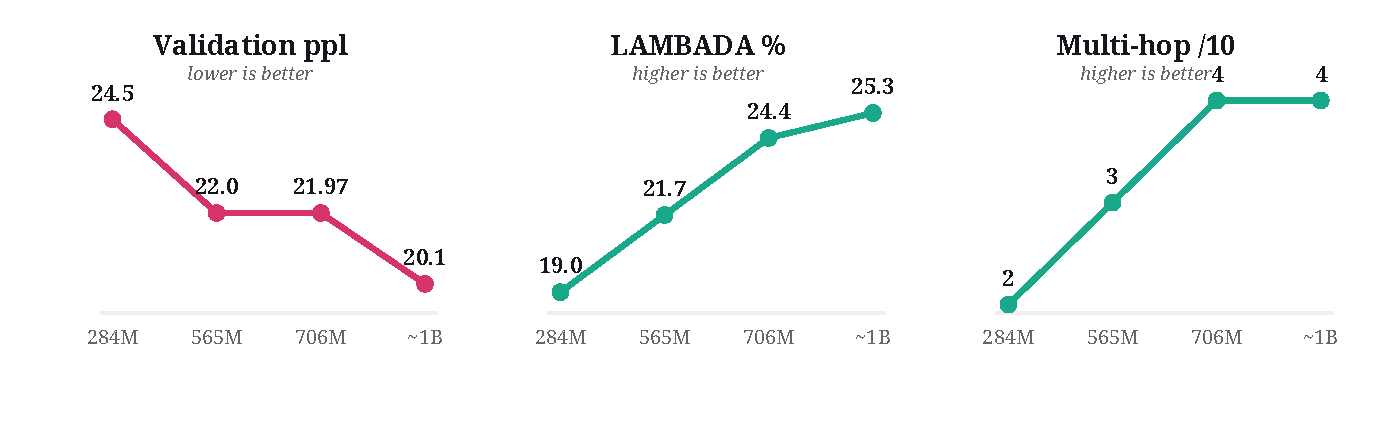
\includegraphics[width=\linewidth]{figs/progression.pdf}
\caption{Progression across the four grown sizes. Validation perplexity falls, and LAMBADA (the most fluency-dependent benchmark) and the greedy multi-hop battery both rise monotonically, the design improves consistently as it grows and trains, with the largest gains on the tokens-limited axes.}
\end{figure}

\subsection{A non-controlled external reference (illustrative only)}
A fair objection is that placing a recurrence at the core, rather than attention, might cost multi-hop reasoning specifically, attention's content-addressed retrieval is the natural mechanism for arbitrary hops. We cannot settle this without a same-corpus matched transformer, which is outside our compute budget (\S7). For rough context only, we ran one published open transformer of similar size and token budget, \textbf{Cerebras-GPT-1.3B}, trained \emph{Chinchilla-optimally} (${\sim}20$ tokens/param, close to our 1B's ${\sim}24$), through the identical harness. \textbf{This is a non-controlled comparison}: tokenizer, corpus, optimizer, batch size, and recipe all differ, so we draw no architectural conclusion from it and report it only as illustration.

\begin{table}[h]\centering\small
\caption{Our 1B (spin-dominant) vs a roughly token-matched transformer. On the multi-hop task (ARC-Challenge) both sit at chance; the transformer's lead is concentrated on general-English fluency, where our custom corpus and tokenizer are confounds.}
\begin{tabular}{@{}l r r r r r r@{}}
\toprule
Model & Params & PIQA & ARC-E & ARC-C & HellaSwag & LAMBADA \\
\midrule
\textbf{Pragnosia (ours, spin)} & 1022M & 63.3 & 37.2 & 24.3 & 29.6 & 25.3 \\
Cerebras-GPT-1.3B (transformer) & 1316M & 67.1 & 38.9 & 25.7 & 35.9 & 47.0 \\
\bottomrule
\end{tabular}
\end{table}

Read with that caveat, one observation is at least \emph{consistent} with a scale (not architecture) reading of the multi-hop weakness: on \textbf{ARC-Challenge both models sit at chance} (24.3 and 25.7 vs 25\%), the reference transformer reasons no better at this scale either, and on ARC-Easy the two are within 1.7 points. The reference is ahead on general-English fluency (LAMBADA, HellaSwag), which is exactly where its larger size, general-web corpus, and standard tokenizer would help against our smaller, reasoning-heavy, custom-BPE setup. We stress again that none of this is controlled and none of it is evidence \emph{for} the design; the claim we actually stand on is the causal one, which needs no baseline.

\section{Comparison with Large Language Models}
\begin{table}[h]\centering\small
\caption{Where each paradigm wins. The two are built on opposite bets.}
\begin{tabular}{@{}p{4.3cm} p{4.0cm} p{6.0cm}@{}}
\toprule
Property & Today's LLMs & Pragnosia \\
\midrule
Fluent language / world knowledge & Strong / vast & Decent / limited (small) \\
Reasoning depth & Strong & Single-step real, multi-hop weak \\
Long-context / inference cost & $O(T^2)$, KV-cache grows & $O(T\cdot d)$, recurrent $O(1)$/token (realized at 706M; carry helps for aggregate context; sharp retrieval still weak, \S8 v) \\
Learn after training, no retrain & No (frozen) & Yes (replay + plasticity) \\
Forgetting on update & Catastrophic & Low (generative replay) \\
Self-paced learning rate & Fixed schedule & Surprise-modulated \\
Hand-set behavior & & None (self-derived) \\
Knows what it doesn't know & Partial, bolted on & Abstains, but signal scale-limited \\
Size / cost & Data-center & Single laptop GPU \\
\bottomrule
\end{tabular}
\end{table}

\section{Limitations}
Every claim above carries a number; the open frontier is equally explicit. (i) \textbf{The decisive at-scale experiment is missing, and the headline rests on one seed.} We separate two claims: the \emph{quality} win (spin-dominant beats a matched transformer) is shown at ${\approx}37$M, 3 seeds; the \emph{causal-dominance} property (the carrier is load-bearing) is shown at 284M, one seed. These are not the same claim, and the $306\times$ number shows the carrier is \emph{used}, not that the design \emph{wins} at scale. The single highest-value experiment, a \code{carrier="none"} transformer at 284M, same corpus and budget, is what would join them; it is not a footnote but the crux, and it is still to run. The asymmetry is also backwards from ideal: the cheap result is replicated (3 seeds) and the expensive headline is not, so a second 284M seed (even at reduced budget) is needed to know whether $306\times$ is stable. Crucially, the causal-dominance property itself does \emph{not} need a baseline, and it \textbf{persists and strengthens across scale}: carrier ablation costs \textbf{$306\times$ at 284M, $1081\times$ at 706M, and $1886\times$ at 1B} (a 1.0B spin-dominant model grown function-preservingly from the 706M, val ppl ${\sim}17.8$). This within-model scaling is a meaningful result on its own, as the model grows, the carrier becomes \emph{more} load-bearing, not less. A matched \emph{transformer} at 1B is outside our available compute budget and we do not claim it; the matched \code{carrier="none"} transformer at \textbf{284M} is the one we can afford and is the crux for the separate \emph{quality} claim. (ii) \textbf{The models are undertrained for their grown size, and we treat this as a claim to be falsified, not a shield.} Single-step reasoning, arithmetic, and fact recall are real; multi-hop composition (relational analogy, multi-step deduction, counterfactual and causal chains) is weak. Our best evidence that tokens are the lever is the 565M: more training raised the most fluency-dependent task most (LAMBADA $19.0\to21.7$). A direct 2-point check on the multi-hop axis itself (284M vs 565M, greedy battery of analogy / multi-step / counterfactual / causal) nudges $2/10 \to 3/10$, the gain in counterfactual, while analogy and causal stay at floor: consistent with the account but within the noise of a 10-item probe. To make this falsifiable rather than convenient, the missing measurement is the full \emph{token-vs-capability curve on the multi-hop axis}; if more tokens do not move it, the undertraining account is wrong, and we will report it. (iii) \textbf{Honesty is not solved.} The consistency-based gate abstains on the clearly-unknowable but cannot separate knowledge from confident confabulation at 284M (\S5); it needs scale or a redesigned signal. (iv) Like all small models it can be \emph{confidently wrong} on familiar-but-incorrect facts. (v) \textbf{Long context: aggregate use is now realized; sharp retrieval is not.} The carrier is $O(T\cdot d)$ and the windowed-generation path keeps attention positions in-distribution, so the architecture \emph{supports} unbounded context. The realization has a clear arc. A model trained at a fixed 256-token window with each window starting fresh never learns to \emph{use} a cross-window carried state; at 565M, feeding one \emph{hurt} (next-window ppl 62.6 with the carry vs 58.0 without). We then implemented the cross-window state-threading \emph{and} trained with it (a curriculum mixed-window continual schedule that grows the model while keeping the long objective in the replay mix). On the resulting \textbf{706M} model the carry now \emph{helps}: next-window ppl \textbf{21.6 with vs 22.3 without}, and longer effective context lowers perplexity ($W{=}32$: 21.4 vs $W{=}1$: 22.8). So the structural advantage is realized for \emph{aggregate/topical} context (long generations stay on-theme). We verify the inference claim directly on the 1B: greedy and sampled generation both run at a \textbf{constant ${\sim}27$ tokens/s from 256 to 8000 tokens} (the $O(1)$/token property, no KV-cache, at every length). Coherence over that span is \emph{decoding}-dependent, not architectural: greedy repetition-loops by ${\sim}1$k tokens (tail unique-word ratio 0.14, held to 8k), whereas temperature sampling stays varied and on-theme all the way out (0.66 at 8k). The earlier ``it loops past ${\sim}3$k'' was thus a greedy-decoding artifact, not the carrier. What is \emph{not} yet there is \emph{sharp long-range retrieval}: a specific fact ${\sim}300$ tokens back is not reliably recalled, the damped carry provides gist, not verbatim memory. Closing that likely needs full-BPTT write-side training, which we have not run at scale. None of these is hidden.

\section{Conclusion}
Pragnosia is a transformer/SSM hybrid in which a diagonal-complex spin recurrence is the core token-mixer, wrapped in a self-calibrating controller for continual learning, a persistent in-weights episodic memory, an introspection layer, and self-governed growth, with no hand-set constants. The central, honest finding is about \emph{placement}: a single spin carrier drifts to a causally-negligible side-channel as the model scales (0.028\% of the loss at 1.4B), and a parameter-matched ablation shows the intended spin-dominant design, spin as the core mixer, is the most parameter-efficient (219 vs 279 ppl). At 284M, the first at-scale training of the intended build, ablating the carrier costs \textbf{$306\times$} in perplexity versus $3.4\times$ for attention: the spin carrier is the load-bearing core, the exact inverse of the 1.4B drift. The remaining work is a matched transformer baseline and multi-seed replication at 1B, and training the models to their compute-optimal token budget. We release the full system, every measured number, and every limitation.

\bibliographystyle{unsrt}
\bibliography{references}
\end{document}
